\documentclass{beamer}

\mode<presentation> {
\usetheme{Madrid}
\setbeamertemplate{footline}[page number]
\setbeamertemplate{navigation symbols}{}
}

\usepackage{graphicx}
\usepackage{booktabs}
\usepackage{tkz-graph}
\GraphInit[vstyle = Shade]
\tikzset{
  LabelStyle/.style = { rectangle, rounded corners, draw,
                        minimum width = 2em, fill = yellow!50,
                        text = red, font = \bfseries },
  VertexStyle/.append style = { inner sep=5pt,
                                font = \normalsize\bfseries},
  EdgeStyle/.append style = {->, bend left} }
\usetikzlibrary {positioning}
\definecolor {processblue}{cmyk}{0.96,0,0,0}
\definecolor{lightgray}{gray}{0.95}


\title[DNN and MILP]{Deep neural networks and mixed integer linear optimization}
\author{Mateo Fischetti, Jason Jo}
\date{\today}

\begin{document}

\begin{frame}
\titlepage
\end{frame}

\begin{frame}
\frametitle{Overview}
\tableofcontents
\end{frame}

\section{Introduction}
\begin{frame}{Introduction}
  \begin{itemize}
  \item Deep Neural Networks (DNN) are composed of layers of neurons
  \item Each neuron calculates an affine combination of the outputs of the previous layer;
  \item Finally, each neuron applies a non-linear operator on the result and feeds it to the next layer
    \begin{itemize}
    \item A common operator is the ReLU function
    \end{itemize}
  \end{itemize}
\end{frame}

\section{Definitions}
\begin{frame}{Definitions}
  \begin{itemize}
  \item A DNN is composed of $K+1$ layers, numbered $0$ to $K$
    \begin{itemize}
    \item Layer $0$ is a ``fake'' layer, and consists of the input of the network
    \item Layer $N$ is the output of the network
    \end{itemize}
  \item Each layer $k$ is composed of $n_k$ neurons (or units), numbered from $1$ to $n_k$
  \end{itemize}
\end{frame}

\begin{frame}{Definitions}
  \begin{itemize}
  \item Let $x_k \in \mathbb{R}^{n_k}$ be the output vector of layer $k$, and $x^j_k$ is the scalar output of \texttt{UNIT}$(j,k)$
  \item For each layer $k \geq 1$, \texttt{UNIT}$(j,k)$ computes its output vector using the following formula:
  \end{itemize}
  $$
  x^k = \sigma(W^{k-1} x^{k-1} + b^{k-1})
  $$
  \begin{itemize}
  \item where $\sigma(.)$ is a non-linear function, $W^{k-1}$ and $b^{k-1}$ are a matrix of weights and a vector of activation biases
    \begin{itemize}
    \item One possible operator is the ReLU~(rectified linear unit) function
    \end{itemize}
  \end{itemize}
\end{frame}

\begin{frame}{Proposal}
\begin{itemize}
    \item Use $W^k$ and $b^k$, $\forall k \in [0, K]$ to build an optimization model for adversarial examples generation
    \item Problem: $\sigma(.)$ is not linear
\end{itemize}
\end{frame}

\begin{frame}{Proposal}
\begin{itemize}
    \item Use $W^k$ and $b^k$, $\forall k \in [0, K]$ to build an optimization model for adversarial examples generation
    \item Problem: $\sigma(.)$ is not linear
\end{itemize}
\end{frame}

\begin{frame}{ReLU Operator}
  $$ \text{ReLU}(x) = \text{max}(0, x) $$
  \begin{figure}[H]
    \centering
    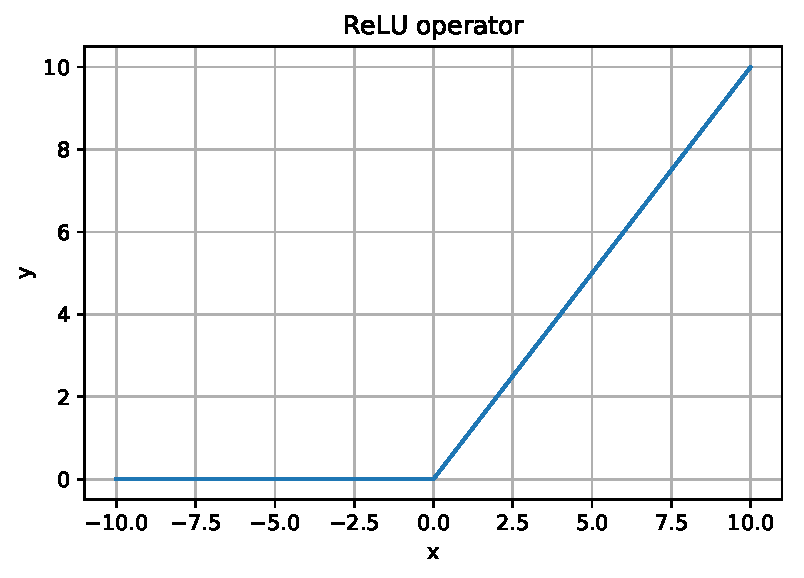
\includegraphics[width=0.8\columnwidth]{relu}
  \end{figure}
\end{frame}

\begin{frame}{Problem}
  ReLU $ \rightarrow $ not a linear function
\end{frame}

\begin{frame}
  \Huge{\centerline{Fin}}
\end{frame}

\end{document}